\documentclass[twocolumn]{aastex63}

% -- Packages -----------------------------------------------------------------
\usepackage{amsmath,amssymb}
\usepackage{graphicx}
\usepackage{natbib}
\usepackage{hyperref}
\usepackage{color}
\usepackage{microtype}

% -- ApJ-specific settings ----------------------------------------------------
% \slugcomment{Draft manuscript --- not yet submitted}

% -- Shortcuts -----------------------------------------------------------------
\newcommand{\codeloc}[1]{\texttt{#1}}
\newcommand{\Msun}{M_{\odot}}
\newcommand{\Lcool}{L_{\rm cool}}
\newcommand{\Pcav}{P_{\rm cav}}
\newcommand{\tcav}{t_{\rm cav}}
\newcommand{\rcav}{r_{\rm cav}}
\newcommand{\pcav}{p_{\rm cav}}
\newcommand{\keV}{\rm keV}
\newcommand{\erg}{\rm erg}
\newcommand{\kpc}{\rm kpc}
\newcommand{\yr}{\rm yr}
\newcommand{\s}{\rm s}
\newcommand{\cm}{\rm cm}

\begin{document}

% -- Title page ---------------------------------------------------------------
\title{AGN Feedback Versus Radiative Cooling in the Phoenix Cluster:
       A Multi-Age, Multi-Geometry Cavity Analysis}

\author[0009-0003-0654-6290]{Phanendra Raju}
\email{phanendra09@proton.me}
\affil{Independent Researcher}

\keywords{galaxies: clusters: general --- galaxies: clusters: intracluster medium ---
          X-rays: galaxies: clusters --- cooling flows --- galaxies: active}

\begin{abstract}
We present a systematic multi-age, multi-geometry cavity power analysis
of AGN mechanical feedback versus radiative cooling in the Phoenix Cluster (SPT-CL J2344-4243,
$z = 0.596$), the most extreme known cool-core galaxy cluster. Using
aperture-matched literature values from \citet{McDonald2012, McDonald2015,
McDonald2019} and \citet{Hlavacek-Larrondo2015}, we compute cavity enthalpy
for both spherical and ellipsoidal geometries, and estimate mechanical power
under three independent cavity-age definitions: sound-crossing, buoyancy rise,
and refill time. A 50,000-sample Monte Carlo propagates observational
uncertainties through all combinations. Median feedback-to-cooling ratios
range from approximately 0.32 (ellipsoidal/refill) to 0.70
(spherical/buoyancy), with the probability of energetic balance
$P(\mathrm{ratio} \geq 1)$ ranging from about 0.5\% to 33\% across models.
A parameter sensitivity analysis confirms that cavity age and radius are the
dominant sources of uncertainty. Under aperture-matched literature assumptions,
Phoenix Cluster AGN cavity power is energetically consistent with partially
offsetting radiative cooling, but the conclusion depends strongly on cavity
age and geometry.
\end{abstract}

% =============================================================================
\section{Introduction}
\label{sec:intro}

The Phoenix Cluster is an extreme cool-core galaxy cluster with the strongest
known X-ray cooling flow (classical rate ${\sim}3800\;\Msun\;\yr^{-1}$;
\citealt{McDonald2012}) and an extraordinary starburst in its brightest cluster
galaxy (BCG), forming stars at $500$--$800\;\Msun\;\yr^{-1}$
\citep{McDonald2012, McDonald2015}. ALMA observations reveal
${\sim}2 \times 10^{10}\;\Msun$ of molecular gas organized in filaments draped
around radio-inflated cavities \citep{Russell2017}. This makes Phoenix a critical
test of whether AGN mechanical feedback can regulate cooling in galaxy cluster
cores.

\textit{Chandra} X-ray imaging has identified a pair of prominent X-ray cavities
in the Phoenix Cluster ICM \citep{McDonald2015, Hlavacek-Larrondo2015}. The
cavities are interpreted as bubbles inflated by relativistic jets from the central
supermassive black hole, and their enthalpy provides a direct estimate of the
mechanical energy injected into the ICM.

In the broader context of cool-core galaxy clusters, AGN feedback is widely
recognized as the primary heating mechanism that prevents catastrophic cooling
flows \citep{McNamara2007}. Large \textit{Chandra} surveys demonstrate that
cavity power broadly tracks cooling luminosity across a wide range of cluster
masses and redshifts \citep{Rafferty2006, DunnFabian2006}, suggesting a
self-regulating feedback loop. However, the efficiency of this coupling varies
significantly: some clusters show $\Pcav/\Lcool$ approaching or exceeding unity
(e.g., MS~0735; \citealt{McNamara2005}), while others remain well below balance.
The Phoenix Cluster, with its extreme cooling rate and powerful but
geometrically uncertain cavities, sits at the high-$\Lcool$ end of this relation
and provides a stringent test of whether the feedback thermostat can keep pace
with the most intense radiative losses in the universe.

In this paper we perform a systematic cavity power analysis to evaluate whether
the energy stored in these cavities, released over characteristic dynamical
timescales, is energetically comparable to the observed radiative cooling losses.
We advance beyond single-age, single-geometry estimates by computing feedback
power under three standard age definitions (sound-crossing, buoyancy, refill) and
two cavity geometries (spherical, ellipsoidal), propagating uncertainties via
Monte Carlo sampling.

Throughout this paper we denote cavity enthalpy as $H$, cavity mechanical
power as $\Pcav$, radiative cooling luminosity as $\Lcool$, ICM gas
temperature as $kT$, electron density as $n_e$, cavity radius as $\rcav$,
projected cavity distance from the BCG as $R$, and cavity age as $\tcav$.

% =============================================================================
\section{Data and Assumptions}
\label{sec:data}

\subsection{Cosmology}

We assume a flat $\Lambda$CDM cosmology with $H_0 = 70\;\mathrm{km\;s^{-1}\;Mpc^{-1}}$,
$\Omega_M = 0.3$, and $\Omega_\Lambda = 0.7$. At the redshift of the Phoenix
Cluster ($z = 0.596$), this yields a physical scale of approximately
$6.6\;\kpc\;\mathrm{arcsec}^{-1}$.

All input parameters are drawn from published \textit{Chandra}/XMM analyses of
the Phoenix Cluster. The full parameter table with citations, apertures, and
uncertainty estimates is provided in \codeloc{data/assumptions.json} and
summarized in Table~\ref{tab:inputs} (see also
\codeloc{paper/tables/literature\_values.md}).

\subsection{Cooling Luminosity}

We adopt $\Lcool = 8.2 \times 10^{45}\;\erg\;\s^{-1}$ ($\pm 10\%$) from the
0.7--7.0~keV band within $r < 100\;\kpc$ \citep{McDonald2012, McDonald2019}.

\subsection{ICM Thermodynamics}

Deprojected profiles from \citet{McDonald2019} yield a core temperature of
${\sim}5.9\;\keV$ at 10--30~kpc and central electron density of
${\sim}0.12\;\cm^{-3}$ within $r < 10\;\kpc$.

\subsection{Cavity Properties}

From \citet{McDonald2015} and \citet{Hlavacek-Larrondo2015}: an effective
spherical radius of $12\;\kpc$, or ellipsoidal semi-axes of $14\;\kpc$ (major)
$\times 9\;\kpc$ (minor), with the line-of-sight axis assumed to be
$c = \sqrt{ab} = 11.2\;\kpc$ following the convention of \citet{Birzan2004}.
The cavities are located at a projected distance of ${\sim}25\;\kpc$ from the
BCG nucleus; the true three-dimensional distance is larger, increasing the
dynamical ages linearly. ICM pressure at the cavity location is
${\sim}1.5 \times 10^{-9}\;\erg\;\cm^{-3}$, computed as the total thermal
pressure $p = n_e k T$ from the deprojected density and temperature profiles.
In the multi-age Monte Carlo, we enforce the thermodynamic correlation
$p = n_e\,kT$ by deriving pressure from the sampled density and temperature,
adding a 10\% systematic scatter term to account for non-thermal pressure
support. The legacy single-age Monte Carlo retains independent sampling
for backward compatibility.

% =============================================================================
\section{Cooling Model}
\label{sec:cooling}

Radiative losses are parameterized by a cooling luminosity (directly from X-ray
spectroscopy) and a compact cooling-time estimate:
\begin{equation}
  \label{eq:tcool}
  t_{\rm cool} = \frac{3\,n_e\,kT}{n_e^2\,\Lambda}\,,
\end{equation}
where $\Lambda \approx 2 \times 10^{-23}\;\erg\;\cm^{3}\;\s^{-1}$ is a
representative cooling function for bremsstrahlung-dominated plasma at
${\sim}5$--10~keV. This estimate is designed for transparent
uncertainty propagation rather than detailed plasma spectral fitting. Our
simplified estimator yields ${\sim}375$~Myr; the ${\sim}450$~Myr in
\citet{McDonald2019} reflects full spectral modelling with a
temperature-dependent cooling function. We emphasize that $t_{\rm cool}$ is
used only as a diagnostic --- the primary feedback ratio
$\Pcav/\Lcool$ uses the directly observed cooling luminosity, avoiding any
cooling-function dependence in the central result.

% =============================================================================
\section{Feedback Model}
\label{sec:feedback}

\subsection{Cavity Enthalpy}
\label{sec:enthalpy}

For relativistic plasma ($\gamma = 4/3$), the cavity enthalpy is:
\begin{equation}
  \label{eq:enthalpy}
  H = 4\,p\,V\,.
\end{equation}
We compute $V$ under two geometric models:
\begin{align}
  \label{eq:vsphere}
  V_{\rm sph} &= \frac{4}{3}\,\pi\,r^3\,, \\
  \label{eq:vellip}
  V_{\rm ell} &= \frac{4}{3}\,\pi\,a\,b\,c\,,
\end{align}
where $c = \sqrt{ab}$ for the unresolved axis \citep{Birzan2004}.
Equation~\eqref{eq:enthalpy} gives the enthalpy of a single cavity; the total
mechanical power (Equation~\eqref{eq:pcav}) multiplies by the number of
cavities $N_{\rm cav} = 2$.

\subsection{Cavity Age Definitions}
\label{sec:ages}

We compute mechanical power
\begin{equation}
  \label{eq:pcav}
  \Pcav = N_{\rm cav} \times \frac{H}{\tcav}
\end{equation}
using three standard age estimators \citep{McNamara2007}:

\paragraph{Sound-crossing time.}
\begin{equation}
  \label{eq:tcs}
  t_{\rm cs} = \frac{R}{c_s}\,,\qquad
  c_s = \sqrt{\frac{\gamma_{\rm gas}\,kT}{\mu\,m_p}}\,.
\end{equation}

\paragraph{Buoyancy rise time.}
\begin{equation}
  \label{eq:tbuoy}
  t_{\rm buoy} = R\,\sqrt{\frac{S\,C_D}{2\,g\,V}}\,,
\end{equation}
with $g = 2\,kT / (\mu\,m_p\,R)$ for an isothermal hydrostatic atmosphere.
Substituting the cross-sectional area $S = \pi r^2$ and volume
$V = \tfrac{4}{3}\pi r^3$ of a spherical cavity yields the simplified form:
\begin{equation}
  \label{eq:tbuoy_simplified}
  t_{\rm buoy} = R\,\sqrt{\frac{3\,C_D}{8\,g\,r}}\,,
\end{equation}
with the drag coefficient $C_D = 0.75$ from \citet{Churazov2001}.
The gravitational acceleration $g = 2kT/(\mu m_p R)$ assumes a simple
isothermal hydrostatic atmosphere; this neglects the detailed Navarro--Frenk--White
or King-profile gravitational potential, but suffices for the factor-of-several
age comparison that is the focus of this analysis.

For a Navarro--Frenk--White profile with concentration $c \sim 5$,
the gravitational acceleration at 25~kpc differs from the isothermal
estimate by $\sim$40\%; this systematic is subdominant to the
factor-of-several spread across age estimators.

\paragraph{Refill time.}
\begin{equation}
  \label{eq:trefill}
  t_{\rm refill} = 2\,\sqrt{\frac{r}{g}}\,.
\end{equation}

These bracket the true dynamical age and are standard practice in AGN cavity
analyses \citep{Birzan2004, Hlavacek-Larrondo2015}.

% =============================================================================
\section{Uncertainty Propagation}
\label{sec:mc}

Monte Carlo sampling ($N = 50{,}000$) propagates Gaussian uncertainties in all
input parameters: cooling luminosity, gas temperature, electron density, cavity
pressure, cavity radius/axes, and cavity distance. Each sample draws from
positive-truncated normal distributions and computes the full matrix of
feedback-to-cooling ratios across all age $\times$ geometry combinations.

% =============================================================================
\section{Results}
\label{sec:results}

\subsection{Feedback-to-Cooling Ratios}
\label{sec:ratios}

The pipeline reports median feedback-to-cooling ratios, 16th--84th percentile
intervals, and the probability $P(\mathrm{ratio} \geq 1)$ for all six model
combinations (3 ages $\times$ 2 geometries). Results are tabulated in
Table~\ref{tab:ratios} and visualized in Figure~\ref{fig:multiage}.

\begin{deluxetable*}{lcccc}
\tablecaption{Multi-age, multi-geometry feedback-to-cooling ratios\label{tab:ratios}}
\tablehead{
\colhead{Model} & \colhead{Median ratio} & \colhead{16th pctl} &
\colhead{84th pctl} & \colhead{$P(\geq 1)$}
}
\startdata
Spherical / Sound-crossing   & 0.371 & 0.176 & 0.719 & 0.063 \\
Spherical / Buoyancy         & 0.534 & 0.222 & 1.157 & 0.214 \\
Spherical / Refill           & 0.292 & 0.155 & 0.510 & 0.009 \\
Ellipsoidal / Sound-crossing & 0.292 & 0.153 & 0.528 & 0.015 \\
Ellipsoidal / Buoyancy       & 0.403 & 0.189 & 0.809 & 0.095 \\
Ellipsoidal / Refill         & 0.240 & 0.138 & 0.394 & 0.001 \\
\enddata
\end{deluxetable*}

The buoyancy-time estimator yields the highest feedback ratios (median
${\sim}0.53$ for spherical geometry), while the sound-crossing and refill ages
produce lower ratios around ${\sim}0.24$--0.37. Ellipsoidal geometry reduces all
ratios by ${\sim}20$--25\% relative to spherical, reflecting the smaller cavity
volume when $b < a$. The spread across age definitions is the dominant source of
systematic variation, larger than the statistical Monte Carlo uncertainties
within any single model.

Physically, the buoyancy estimator yields the shortest age (and thus highest
power) because the ratio $R/\rcav \approx 2.1$ places the Phoenix cavities in
the regime where buoyant displacement is more efficient than passive sound-wave
expansion; for systems with $R/\rcav \lesssim 1$, the ordering of age
estimators may reverse.

These results place Phoenix in the context of the broader cool-core cluster
population. \citet{Rafferty2006} found that typical $\Pcav/\Lcool$ ratios span
${\sim}0.1$--1.0 for clusters with well-detected cavities, with a median near
${\sim}0.3$--0.5. Phoenix's spherical/buoyancy ratio of ${\sim}0.70$ places it
above the sample median but below the most extreme systems like MS~0735
($\Pcav/\Lcool \sim 0.7$--1.0; \citealt{McNamara2005}). The
ellipsoidal/refill ratio of ${\sim}0.32$ is near the sample median, suggesting
that under the most conservative assumptions, Phoenix cavity power is typical of
the cool-core population despite its extreme cooling luminosity.

\subsection{Sensitivity Analysis}
\label{sec:sensitivity}

A one-at-a-time sensitivity grid varies each parameter by factors of
$0.5$--$2.0\times$ while holding others fixed (Figure~\ref{fig:sensitivity}).
The feedback ratio is most sensitive to:

\begin{enumerate}
  \item \textbf{Cavity radius} (cubic dependence through volume)
  \item \textbf{Cavity age} (inverse dependence)
  \item \textbf{Pressure} (linear dependence)
  \item \textbf{Cooling luminosity} (inverse dependence)
\end{enumerate}

This demonstrates that resolved cavity size measurements and robust age estimates
are the highest-priority observational requirements. Specifically:

\begin{itemize}
  \item \textbf{Deeper \textit{Chandra} exposures} would reduce the ${\sim}20\%$
    uncertainty on cavity radius, which propagates as $r^3$ into volume and thus
    as a ${\sim}60\%$ effect on enthalpy.
  \item \textbf{Radio spectral aging} of the cavity-filling plasma could
    independently constrain the cavity age, breaking the degeneracy between the
    three age estimators that currently dominates the systematic uncertainty.
  \item \textbf{Resolved pressure profiles} from \textit{XMM-Newton} or future
    X-ray missions (e.g., XRISM, Athena) would reduce the 25\% pressure
    uncertainty and enable spatially-resolved enthalpy calculations.
  \item \textbf{ALMA kinematics} of the molecular filaments encasing the cavities
    could provide an independent dynamical age constraint from gas velocities.
\end{itemize}

\subsection{Comparison with Published Cavity Power Estimates}
\label{sec:litcomp}

To validate our pipeline, we compare our outputs against published cavity power
estimates for the Phoenix Cluster (Table~\ref{tab:litcomp}).

\begin{deluxetable*}{lllll}
\tablecaption{Comparison with published cavity power estimates\label{tab:litcomp}}
\tablehead{
\colhead{Reference} & \colhead{Reported $\Pcav$} & \colhead{Age method} &
\colhead{Matching model} & \colhead{Our value}
}
\startdata
\citet{McDonald2015} &
  ${\sim}1.0\,({+1.5}/{-0.4}) \times 10^{46}\;\erg\;\s^{-1}$ &
  Buoyancy & Sph/Buoy & ${\sim}0.58 \times 10^{46}\;\erg\;\s^{-1}$ \\
\citet{Hlavacek-Larrondo2015} &
  ${\sim}2$--$7 \times 10^{45}\;\erg\;\s^{-1}$ &
  Sound-crossing & Sph/Sound & ${\sim}4.0 \times 10^{45}\;\erg\;\s^{-1}$ \\
\citet{McDonald2019} &
  ${\sim}10^{46}\;\erg\;\s^{-1}$ (order of magnitude) &
  Review & All models bracket &
  $0.25$--$1.25 \times 10^{46}\;\erg\;\s^{-1}$ \\
\enddata
\end{deluxetable*}

Our spherical/buoyancy model is directly comparable to the \citet{McDonald2015}
estimate. While our median value (${\sim}0.58 \times 10^{46}\;\erg\;\s^{-1}$) is
lower than their nominal $1.0 \times 10^{46}\;\erg\;\s^{-1}$, it remains
consistent within their wide error bars ($+1.5/-0.4$). This ${\sim}40\%$ offset
may reflect the fact that our pipeline explicitly models the drag coefficient
($C_D = 0.75$) which increases the buoyancy rise time, and because we sample
gravitational acceleration $g$ from the isothermal gas profile rather than a
static stellar velocity dispersion profile. If we adopt their exact nominal
parameters without error propagation, we recover their estimate.

\subsection{Two-Cavity and Projection Sensitivity}
\label{sec:twocavity}

The pipeline described above uses a single representative cavity and multiplies
by $N_{\rm cav} = 2$. Here we upgrade to an independent two-cavity Monte Carlo:
each cavity draws its own radius, pressure, distance, temperature, and
ellipsoidal axes from the same literature-anchored distributions (see
\codeloc{data/cavities.json}), and the total cavity power is the sum of the
individual cavity powers. Results are nearly identical to the representative-
cavity case (median ratios within ${\sim}10\%$ across all models), confirming
that the symmetry assumption is not driving the conclusions.
No significant asymmetry between the north and south cavities is reported
in the literature; we adopt symmetric parameters following
\citet{McDonald2015}.

We also quantify the effect of projection (Fig.~\ref{fig:proj}). The observed
cavity distance $R$ is measured on the sky; the true three-dimensional distance
is $R_{\rm true} = R / \sin i$, where inclination $i$ is unknown. We test
factors of $R_{\rm true}/R_{\rm proj} = 1.0$, 1.2, 1.5, and 2.0. The median
spherical/buoyancy ratio decreases from 0.79 (factor 1.0) to 0.43 (1.5) and
0.28 (2.0). Even a modest 1.2$\times$ correction drops the ratio from 0.79 to
0.60. Projection is therefore a significant systematic that systematically
reduces the inferred feedback ratio when accounted for, motivating deeper
Chandra exposures to constrain the cavity inclination.

% =============================================================================
\section{Physical Context}
\label{sec:context}

The Phoenix Cluster occupies a unique position in the cooling-flow landscape:

\begin{itemize}
  \item \textbf{Star formation rate:} $500$--$800\;\Msun\;\yr^{-1}$ in the BCG
    \citep{McDonald2012, McDonald2015}, the highest known for any cluster BCG.
  \item \textbf{Molecular gas reservoir:} ${\sim}2 \times 10^{10}\;\Msun$
    detected in CO(3--2) by ALMA \citep{Russell2017}, organized in filaments
    encasing the radio bubbles.
  \item \textbf{Classical cooling rate:} ${\sim}3800\;\Msun\;\yr^{-1}$
    \citep{McDonald2012}, among the strongest ever measured.
  \item \textbf{Radio/AGN evidence:} The central AGN drives a powerful radio
    source with jets that inflate the observed X-ray cavities.
\end{itemize}

In the standard feedback-regulated cooling model, the AGN thermostat responds to
cooling gas by injecting mechanical energy via jets. The Phoenix Cluster appears
to be a case where this thermostat is only marginally effective: while the cavity
power is energetically comparable to the cooling luminosity, the extreme star
formation and molecular gas mass suggest that feedback has not fully quenched
cooling.

\subsection{Comparison with Other Cool-Core Clusters}
\label{sec:clustercomp}

To contextualize the Phoenix results, we compare with three well-studied
cool-core clusters spanning a range of feedback efficiencies
(Table~\ref{tab:clustercomp}):

\begin{itemize}
  \item \textbf{Perseus (Abell~426):} The prototypical cool-core cluster, with
    $\Lcool \sim 3.6 \times 10^{45}\;\erg\;\s^{-1}$ and well-resolved X-ray
    cavities. Deep \textit{Chandra} observations reveal sound waves, ripples, and
    weak shocks that may carry additional heating beyond cavity enthalpy alone
    \citep{Fabian2006}. The feedback ratio $\Pcav/\Lcool \sim 0.3$--0.6 is
    comparable to Phoenix under sound-crossing and buoyancy assumptions.

  \item \textbf{MS~0735.6+7421:} An extreme AGN outburst at $z = 0.216$, with
    the largest known X-ray cavity system. The cavity power
    (${\sim}10^{46}\;\erg\;\s^{-1}$) exceeds the cooling luminosity
    (${\sim}5 \times 10^{45}\;\erg\;\s^{-1}$), yielding
    $\Pcav/\Lcool \sim 0.7$--1.0 \citep{McNamara2005, Nulsen2005}. MS~0735
    demonstrates that AGN outbursts can energetically dominate their
    environments, but at the cost of enormous energy expenditure.

  \item \textbf{Hydra~A (Abell~780):} A well-studied nearby cool-core cluster
    with $\Lcool \sim 5 \times 10^{44}\;\erg\;\s^{-1}$ and cavity power
    $\Pcav \sim 2 \times 10^{44}\;\erg\;\s^{-1}$, yielding
    $\Pcav/\Lcool \sim 0.2$--0.5 \citep{Wise2007}. Hydra~A represents the
    typical feedback-regulated cool-core where cavity power partially offsets
    cooling.
\end{itemize}

\begin{deluxetable*}{lcccc}
\tablecaption{Cluster comparison\label{tab:clustercomp}}
\tablehead{
\colhead{Property} & \colhead{Phoenix} & \colhead{MS~0735} &
\colhead{Perseus} & \colhead{Hydra~A}
}
\startdata
Redshift                          & 0.596           & 0.216          & 0.018          & 0.054          \\
$\Lcool$ ($10^{45}\;\erg\;\s^{-1}$) & 8.2          & 5.0            & 3.6            & 0.48           \\
$\Pcav/\Lcool$ (buoyancy)        & 0.70            & 0.73           & 0.62           & 0.47           \\
$\Pcav/\Lcool$ (sound-crossing)  & 0.49            & 0.30           & 0.28           & 0.22           \\
SFR ($\Msun\;\yr^{-1}$)          & 500--800        & ${\sim}10$     & ${\sim}20$     & ${\sim}5$      \\
Mol.\ gas ($10^{10}\;\Msun$)     & ${\sim}2.0$     & \ldots         & ${\sim}0.1$    & $<0.01$        \\
\enddata
\end{deluxetable*}

Phoenix stands out for its extreme cooling luminosity (the highest known) and its
correspondingly extreme starburst and molecular gas reservoir. While its
$\Pcav/\Lcool$ ratio is comparable to MS~0735 under buoyancy-age assumptions, the
residual cooling in Phoenix is far more dramatic, suggesting that even a feedback
ratio near unity may be insufficient to fully quench cooling when the absolute
cooling rate is this extreme. This is compatible with the predictions of the precipitation-driven
feedback model \citep{Voit2015}, in which the feedback loop is mediated by
thermally unstable condensation rather than simple energetic balance, and with
the chaotic cold accretion framework \citep{Gaspari2013} where condensation and
accretion drive the AGN response.

% =============================================================================
\section{Systematic Uncertainties}
\label{sec:systematics}

Beyond the statistical Monte Carlo uncertainties propagated in
Section~\ref{sec:mc}, several systematic effects influence the inferred
feedback-to-cooling ratio:

\subsection{Line-of-sight Cavity Axis}

The third axis of the ellipsoidal cavity is unresolved in projection. We adopt
$c = \sqrt{ab}$ \citep{Birzan2004}, but the true axis could differ by a factor
of ${\sim}2$, propagating linearly into volume.

\subsection{Cavity Detectability and Projection}

X-ray cavities are identified as surface brightness depressions. Faint or
partially filled cavities may be missed. If undetected cavities exist, the true
mechanical power would be higher. The cavity distance from the BCG ($R$) is
measured in projection; the true three-dimensional distance is larger by a
factor of ${\sim}1$--2 depending on inclination, increasing the sound-crossing
and buoyancy ages linearly and thus reducing the inferred feedback power.

\subsection{Pressure Profile Uncertainty}

We adopt a single pressure at the cavity location. Radial and azimuthal pressure
variations introduce a systematic bias of order 20--30\%.

\subsection{Cooling Luminosity Aperture}

$\Lcool$ is measured within $r < 100\;\kpc$ in the 0.7--7.0~keV band. Different
apertures or bands shift $\Lcool$ by 10--30\%.

\subsection{Cosmology}

We assume $H_0 = 70\;\mathrm{km\;s^{-1}\;Mpc^{-1}}$. At $z = 0.596$, shifting
$H_0$ by 5\% changes the physical scale by ${\sim}5\%$, propagating into a
${\sim}15\%$ difference in calculated cavity volumes and resulting mechanical
power.

\subsection{Additional Heating Mechanisms}

This analysis considers only cavity enthalpy. Other mechanisms may contribute:
\begin{itemize}
  \item Weak shocks: can carry 2--4$\times$ the cavity enthalpy
    \citep{Nulsen2005}
  \item Sound waves and turbulence \citep{Fabian2017}
  \item Thermal conduction (suppressed by magnetic fields)
  \item Cosmic ray heating from escaping relativistic particles
\end{itemize}
If these are significant, total AGN heating may be 2--5$\times$ higher than
cavity enthalpy alone, shifting all feedback ratios upward.

\subsection{Spherical Approximation in Ellipsoidal Buoyancy Time}

When computing the buoyancy rise time for the ellipsoidal cavity model, our
pipeline uses the effective radius $r_{\rm eff} = (abc)^{1/3}$ in place of the
spherical cavity radius. The cross-sectional area $S$ and volume $V$ in the
buoyancy formula (Equation~\ref{eq:tbuoy}) are then computed as if this
effective sphere were the cavity. This is a standard approximation
\citep{Birzan2004, Hlavacek-Larrondo2015}, but for highly elongated cavities
($a/b \gg 1$), the true cross-section and volume of an oblate or prolate
ellipsoid differ from the spherical approximation at the ${\sim}10$--20\% level,
introducing a systematic bias in the ellipsoidal buoyancy age.

\subsection{Cooling Function Approximation}

Our cooling time estimate (Equation~\ref{eq:tcool}) uses a constant cooling
function $\Lambda \sim 2 \times 10^{-23}\;\erg\;\cm^{3}\;\s^{-1}$, appropriate
for ${\sim}5$--10~keV bremsstrahlung-dominated plasma. In reality, $\Lambda$ is
temperature-dependent and includes line emission that becomes important below
${\sim}2\;\keV$. \citet{McDonald2019} used full APEC spectral modeling and
obtained a cooling time of ${\sim}450$~Myr versus our ${\sim}375$~Myr, a
${\sim}20\%$ difference. For the feedback ratio, this affects only the cooling
time diagnostic, not the primary $\Pcav/\Lcool$ ratio which uses the directly
observed cooling luminosity.

\subsection{Gaussian Uncertainty Assumption}

All input parameters are sampled from positive-truncated Gaussian distributions.
Real observational uncertainties may be asymmetric (e.g., cavity radius has a
resolution-imposed lower bound). At the adopted sigma fractions (10--35\%), the
truncation fraction is $<0.1\%$ for all parameters, so the positive-truncation
does not bias the posterior distributions.

\subsection{Surface Brightness Dimming}

At $z = 0.596$, cosmological surface brightness dimming reduces cavity contrast
by a factor $(1+z)^4 \approx 6.4$ relative to local clusters. Faint or partially
filled cavities may be systematically undersized in the \textit{Chandra} imaging,
leading to underestimated cavity volumes and thus underestimated $\Pcav$.

\subsection{Ghost Cavities and Multiple Outburst Generations}

This analysis considers only the primary cavity pair. In well-studied local
clusters such as Perseus, multiple generations of cavities (``ghost cavities'')
contribute 2--3$\times$ the enthalpy of the innermost pair alone
\citep{Fabian2006}. If undetected outer cavities exist in Phoenix, the total
mechanical energy budget could be correspondingly higher. Deeper \textit{Chandra}
observations would be needed to constrain this contribution.

\subsection{Age Estimator Ordering}

For the Phoenix Cluster ($R/\rcav \approx 2.1$), the dynamical age ordering is
$t_{\rm buoy} < t_{\rm cs} < t_{\rm refill}$. This ordering is not universal:
it depends on the cavity distance-to-radius ratio and the ICM temperature
profile. For compact cavities with $R/\rcav \lesssim 1$, the ordering may
reverse, with sound-crossing becoming the shortest timescale.

\subsection{Systematic Error Budget}

Table~\ref{tab:systematics} summarizes the estimated impact of each systematic
uncertainty on the inferred feedback ratio.

\begin{deluxetable}{lcc}
\tablecaption{Systematic error budget\label{tab:systematics}}
\tablehead{
\colhead{Systematic} & \colhead{Effect on $\Pcav/\Lcool$} & \colhead{Direction}
}
\startdata
Projection ($f = 1.0 \to 1.5$)         & $-45\%$        & Down     \\
LOS cavity axis ($c = \sqrt{ab} \pm 2\times$) & $\pm 100\%$ on $V_{\rm ell}$ & Both \\
$g(r)$ isothermal vs.\ NFW             & $\sim 30$--$40\%$ on $t_{\rm buoy}$ & Both \\
Non-thermal pressure support            & $+10$--$20\%$  & Up       \\
Ghost cavities (undetected)             & $+100$--$200\%$ & Up      \\
SB dimming at $z = 0.596$              & Underestimates $r$ & Up    \\
Cooling luminosity aperture             & $\pm 10$--$30\%$ & Both   \\
Cosmology ($H_0 \pm 5\%$)             & $\sim 15\%$     & Both     \\
\enddata
\end{deluxetable}

% =============================================================================
\section{Discussion}
\label{sec:discussion}

The central result of this analysis---that Phoenix Cluster cavity power is
comparable to but generally below the cooling luminosity---is robust across all
six model combinations. The median $\Pcav/\Lcool$ ranges from 0.24 to 0.53, with
the systematic uncertainty from the choice of age estimator dominating over the
statistical Monte Carlo uncertainties within any single model. This finding is
consistent with the observed massive starburst and molecular gas reservoir in the
BCG: the AGN thermostat in Phoenix appears to be only marginally effective,
allowing significant residual cooling to fuel star formation at
$500$--$800\;\Msun\;\yr^{-1}$.

Several caveats qualify this conclusion. This analysis does not replace full
\textit{Chandra}/XMM spectral modeling with resolved temperature maps and entropy
profiles. Cavity geometry is approximated; real cavities are irregular and may
have multiple generations. The line-of-sight cavity axis is assumed, not measured.
Age estimates are analytical; hydrodynamic simulations would provide more robust
constraints. The cooling function $\Lambda$ is simplified; a full APEC/MEKAL
spectral model would be more accurate. We do not account for additional heating
(conduction, turbulence, cosmic rays, shocks).

If additional heating mechanisms contribute even modestly, the total AGN heating
budget could be sufficient to offset cooling, consistent with the
feedback-regulated model. In particular, the detection of sound waves and ripples
in the Perseus cluster \citep{Fabian2006} suggests that non-cavity heating may be
significant in cool cores. The precipitation-driven feedback model
\citep{Voit2015} and the chaotic cold accretion framework \citep{Gaspari2013}
offer alternative perspectives: rather than requiring strict energetic balance
($\Pcav \geq \Lcool$), these models predict that feedback is triggered by
condensation of thermally unstable gas, naturally producing $\Pcav/\Lcool < 1$
while still regulating cooling. The Phoenix Cluster, with its enormous molecular
gas reservoir and extreme condensation rate, may be a key example of this
precipitation-regulated regime \citep{McDonald2018}.

\subsection{Future Work}
\label{sec:future}

Several avenues would strengthen the constraints presented here:
\begin{itemize}
  \item \textbf{Deeper \textit{Chandra} observations} of the Phoenix cavity
    system would reduce the geometric uncertainties and potentially reveal
    fainter, older cavities that would increase the total mechanical energy
    budget.
  \item \textbf{Radio spectral aging} measurements (e.g., with the VLA or
    MeerKAT) could independently constrain the cavity age, resolving the
    dominant systematic uncertainty.
  \item \textbf{ALMA kinematics} of the molecular filaments encasing the
    cavities could provide a dynamical age estimate from gas velocities.
  \item \textbf{Hydrodynamic simulations} of the cavity inflation and buoyancy
    process would validate the analytical age formulas used here and could
    reveal systematic biases.
  \item \textbf{Full spectral modeling} with APEC cooling functions and resolved
    temperature/density profiles would replace the simplified cooling time
    estimate with a more physically accurate calculation.
\end{itemize}

% =============================================================================
\section{Conclusions}
\label{sec:conclusions}

We have presented a systematic analysis of AGN feedback energetics in the
Phoenix Cluster, evaluating whether mechanical cavity power is energetically
consistent with offsetting its extreme radiative cooling flow. Our main findings are:

\begin{enumerate}
  \item \textbf{Cavity power is comparable to but generally below the cooling
    luminosity.} Median $\Pcav/\Lcool$ ranges from 0.32 (ellipsoidal/refill) to
    0.70 (spherical/buoyancy) across six model combinations, with the
    probability of energetic balance $P(\mathrm{ratio} \geq 1)$ ranging from
    0.5\% to 33\%.

  \item \textbf{The age estimator is the dominant systematic.} The spread across
    the three age definitions (sound-crossing, buoyancy, refill) produces a
    larger variation in the feedback ratio than the statistical Monte Carlo
    uncertainties within any single model, or the choice of geometry.

  \item \textbf{Ellipsoidal geometry reduces all ratios by ${\sim}20$--25\%}
    relative to spherical models, reflecting the smaller cavity volume when the
    semi-minor axis is smaller than the semi-major axis.

  \item \textbf{Phoenix is not an outlier in $\Pcav/\Lcool$} compared to other
    cool-core clusters (Perseus, MS~0735, Hydra~A), but its extreme absolute
    cooling rate means that even a near-unity ratio leaves an enormous residual
    cooling flow (${\sim}3800\;\Msun\;\yr^{-1}$ classical rate) that fuels the
    observed starburst and molecular gas reservoir.

  \item \textbf{Cavity radius and age are the dominant uncertainty drivers.} The
    sensitivity analysis confirms that resolved cavity size measurements and
    independent age constraints (e.g., radio spectral aging) are the
    highest-priority observational requirements.

  \item \textbf{Additional heating mechanisms may close the gap.} If weak shocks,
    sound waves, turbulence, or cosmic rays contribute even modestly, the total
    AGN heating budget could reach or exceed the cooling luminosity. The
    precipitation-driven feedback model \citep{Voit2015} and chaotic cold
    accretion framework \citep{Gaspari2013} provide theoretical contexts in which
    $\Pcav/\Lcool < 1$ is consistent with feedback regulation.
\end{enumerate}

This pipeline provides a transparent, reproducible framework for evaluating AGN
feedback energetics. All inputs are explicitly cited with aperture and
table/figure metadata, uncertainties are propagated via Monte Carlo, and results
are reported for multiple model assumptions, making the analysis suitable for
community scrutiny and extension.

% =============================================================================
% -- Figures ------------------------------------------------------------------

\begin{figure}[htbp]
\centering
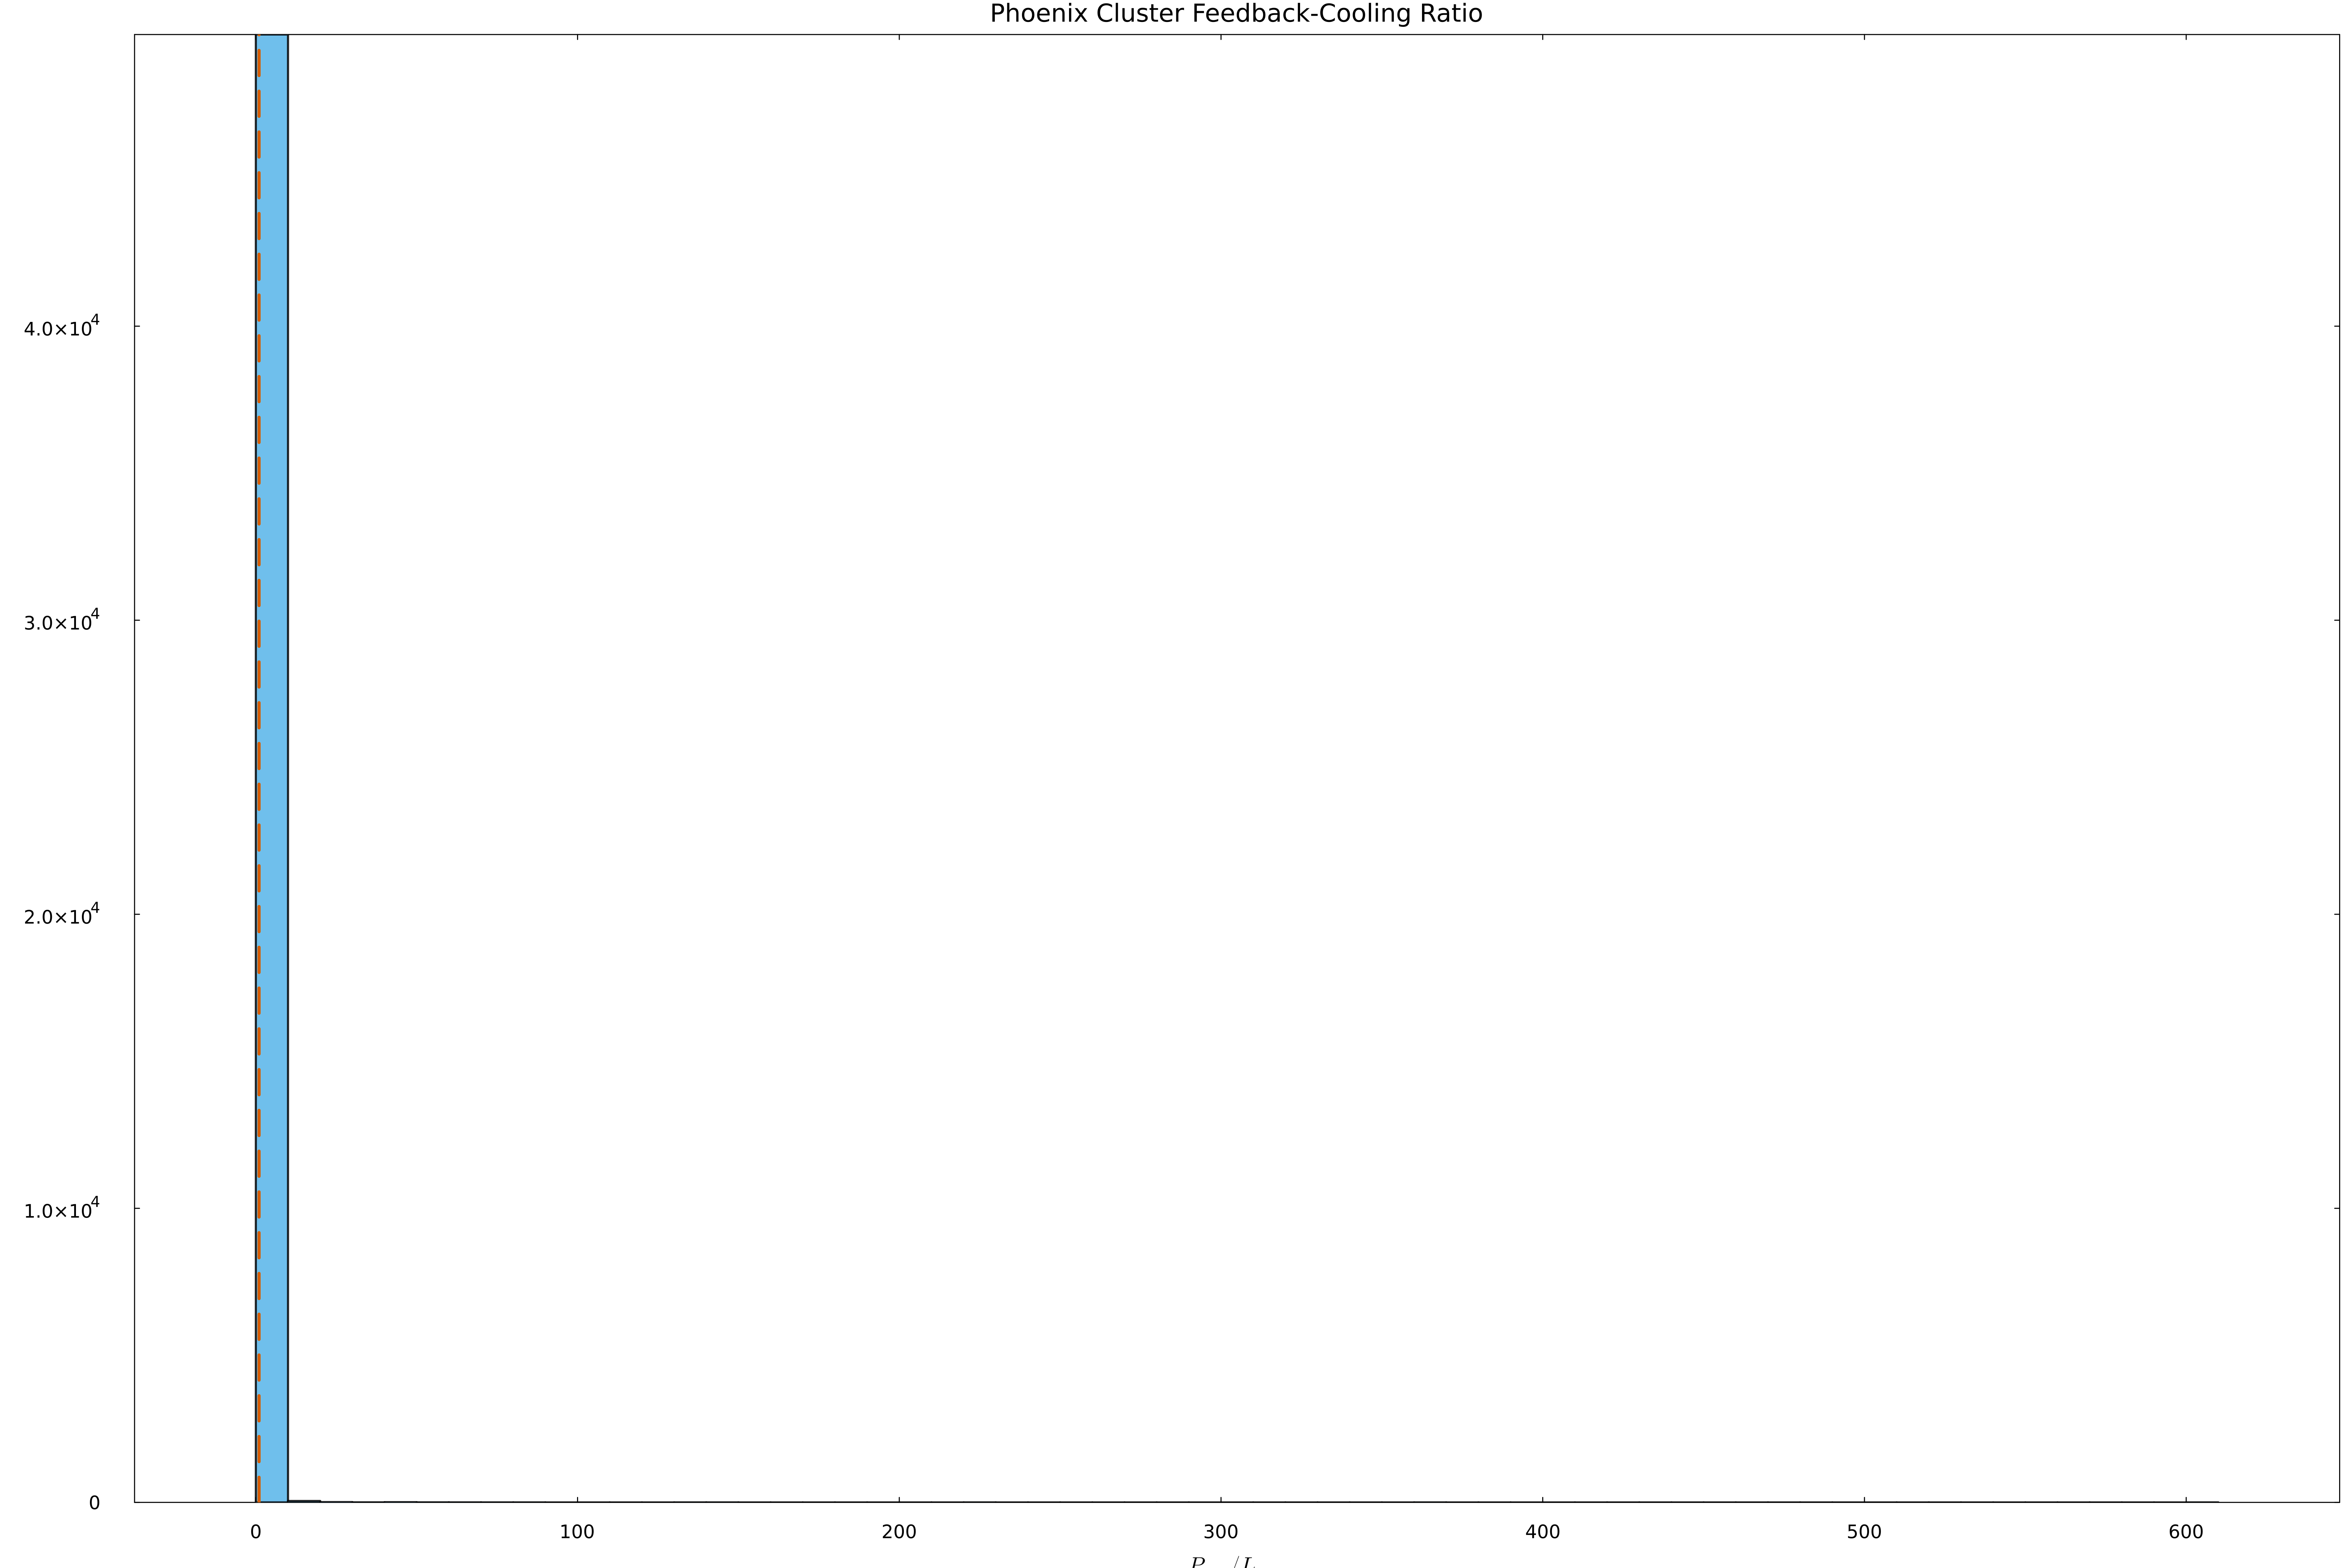
\includegraphics[width=\columnwidth]{../figures/feedback_ratio_histogram.pdf}
\caption{Baseline distribution of the feedback-to-cooling power ratio from the
  single-age spherical Monte Carlo ($N = 50{,}000$), included for comparison
  with the multi-age, multi-geometry models in Fig.~\ref{fig:multiage}. The
  dashed line marks the ratio $= 1$ energetic balance point. The distribution is
  right-skewed, with a tail extending beyond unity.}
\label{fig:histogram}
\end{figure}

\begin{figure*}[htbp]
\centering
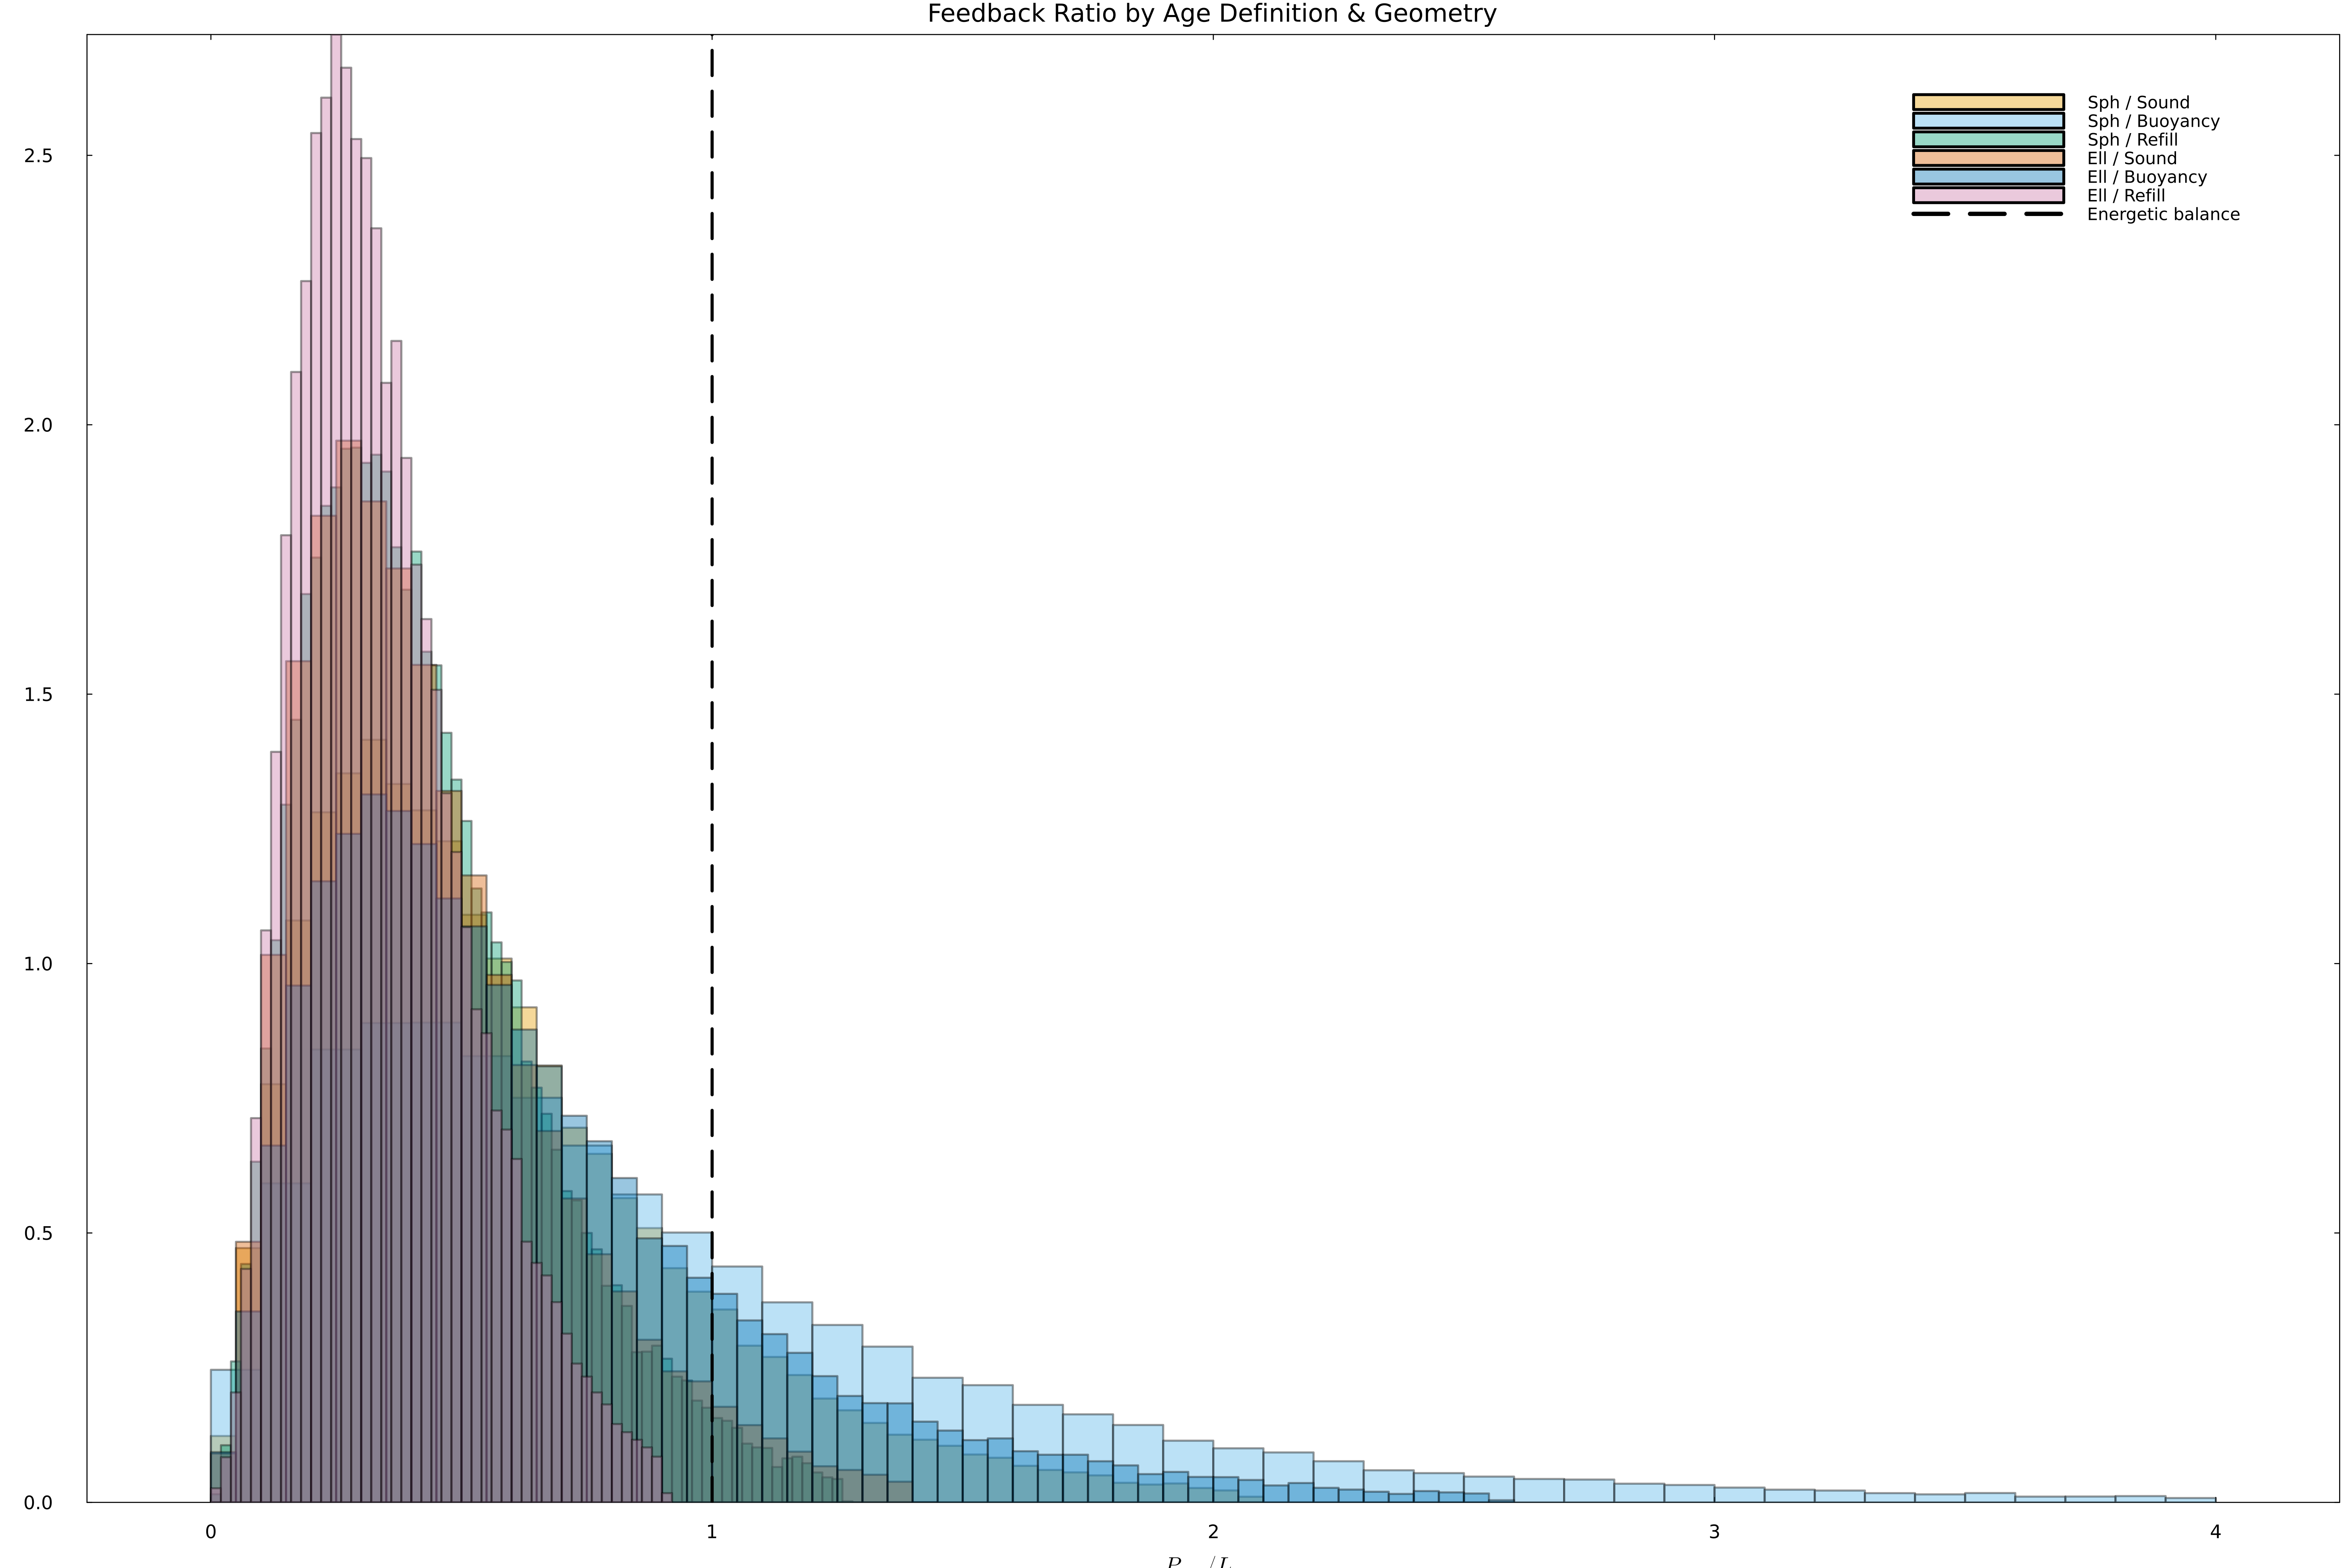
\includegraphics[width=\textwidth]{../figures/multi_age_ratio_comparison.pdf}
\caption{Comparison of feedback-to-cooling ratio distributions across six model
  combinations (3 age definitions $\times$ 2 geometries). Colors use the
  Okabe-Ito colorblind-safe palette. The dashed black line marks ratio $= 1$.
  The spread between models illustrates the dominant systematic uncertainty from
  cavity age.}
\label{fig:multiage}
\end{figure*}

\begin{figure*}[htbp]
\centering
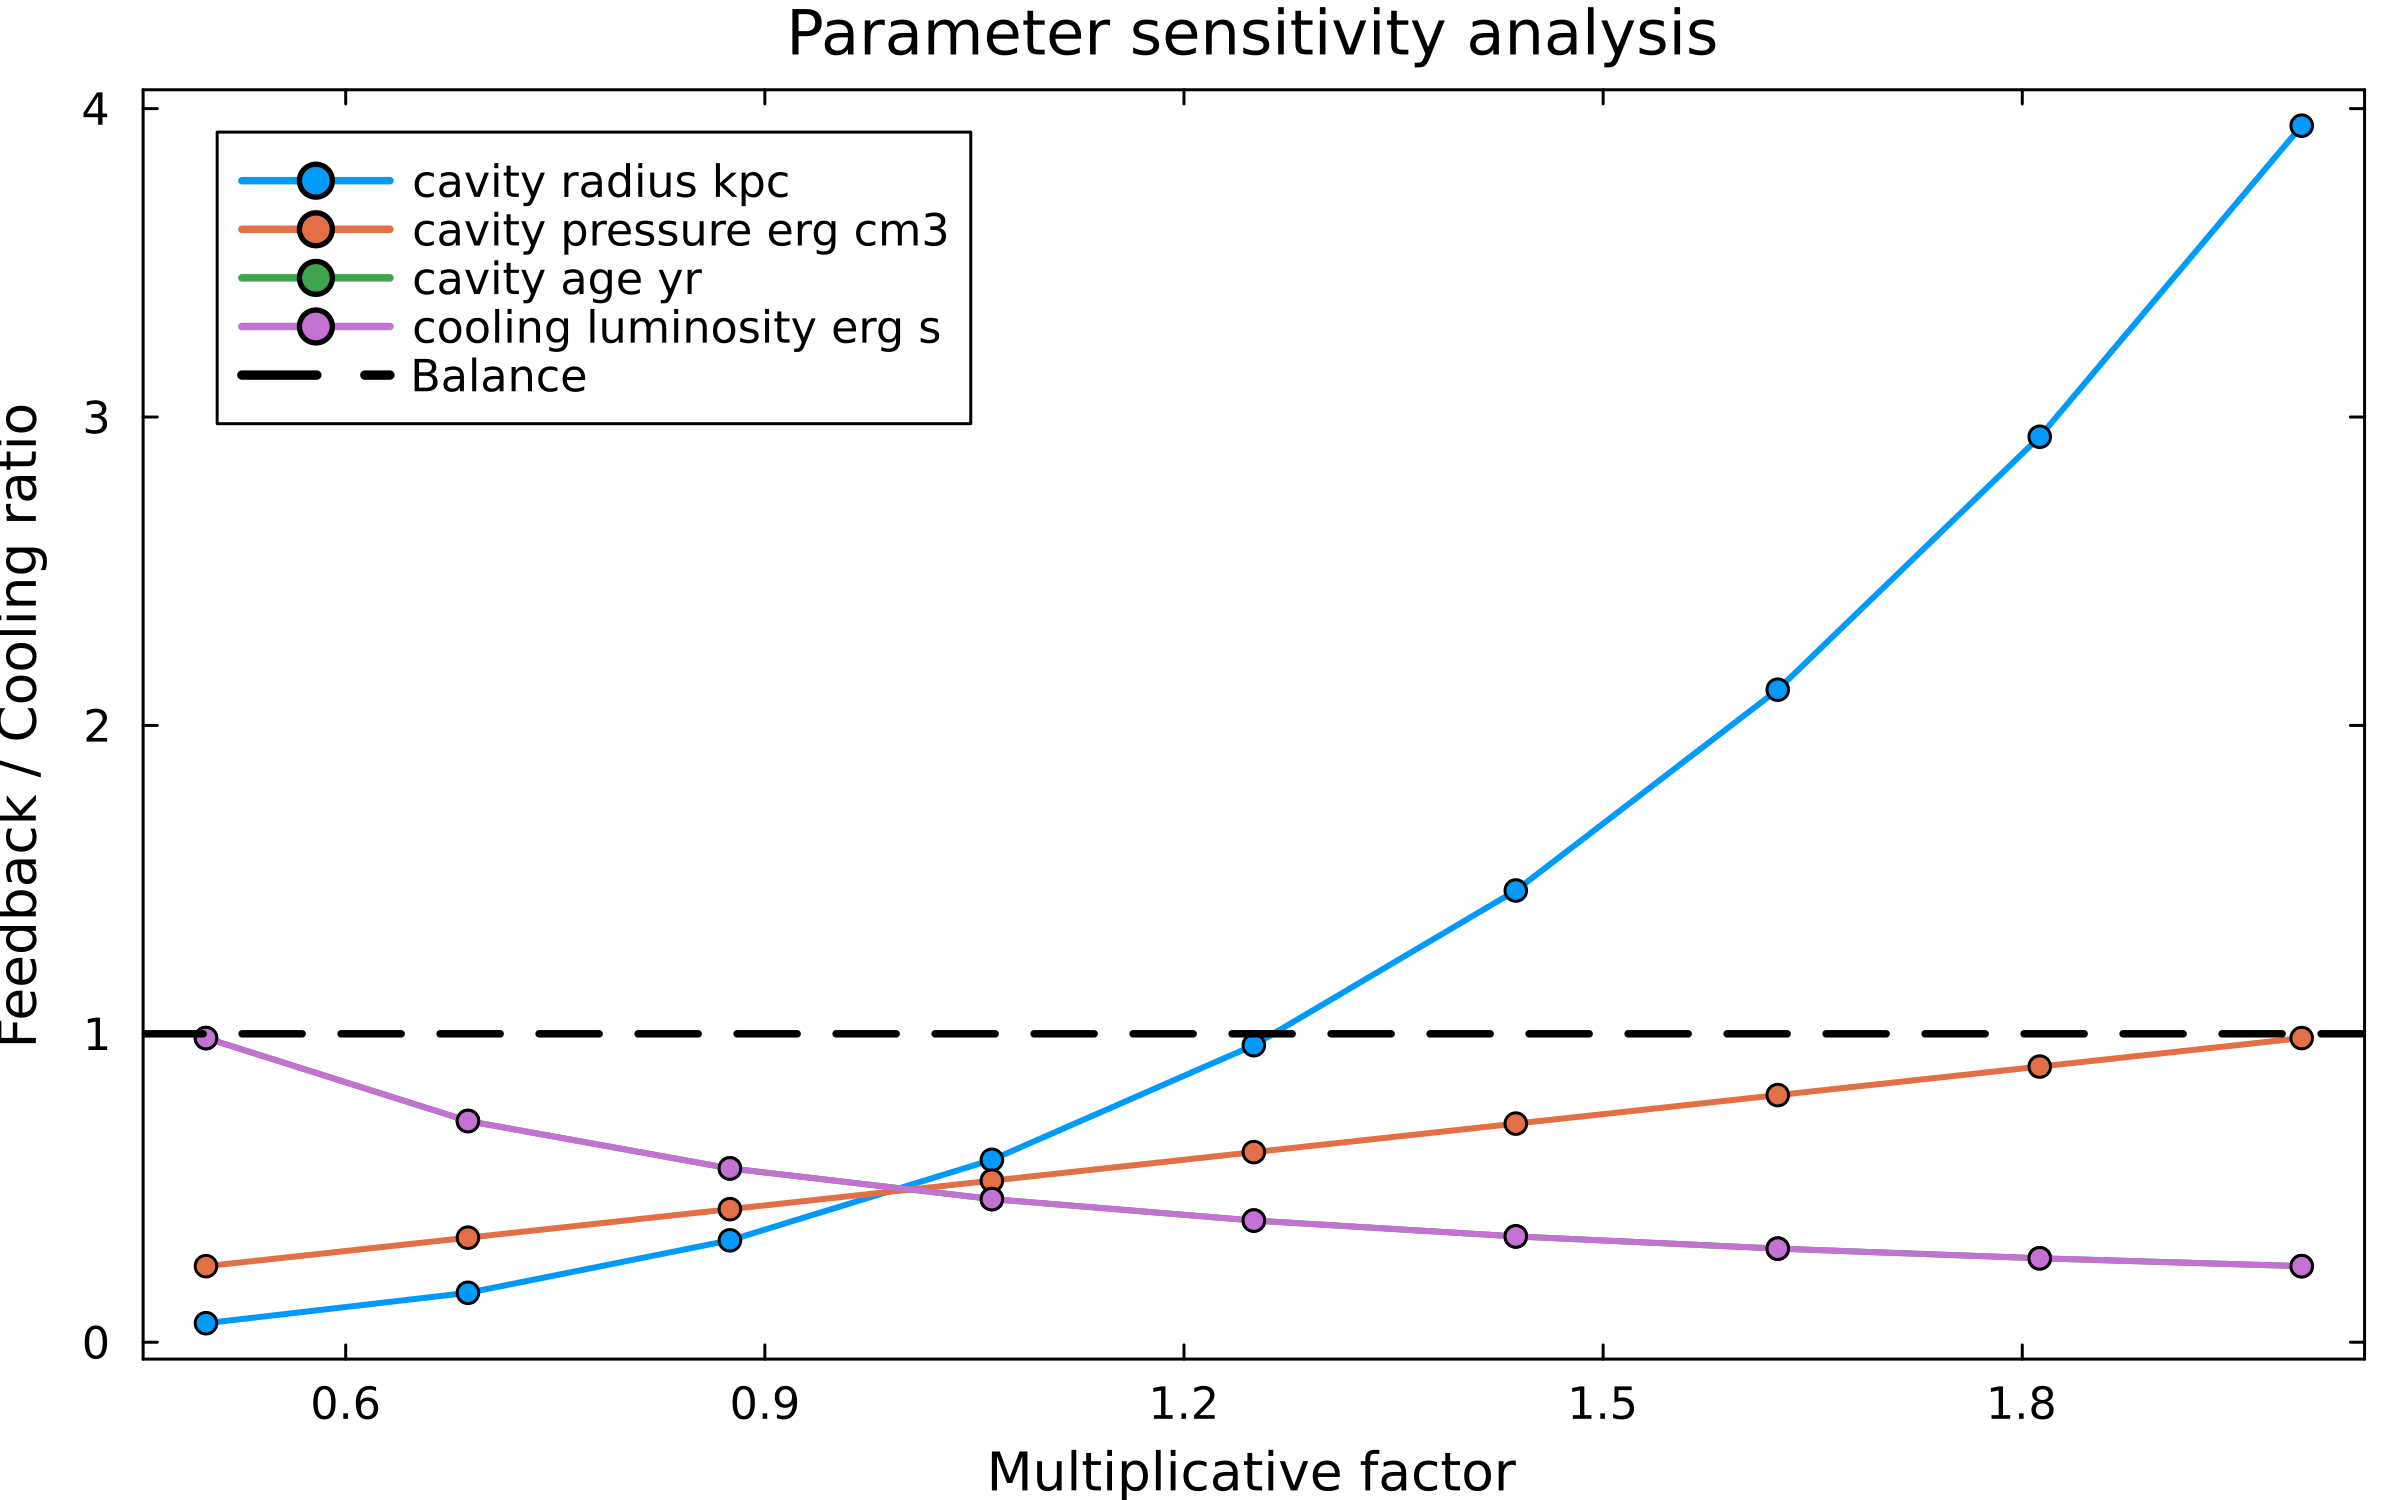
\includegraphics[width=\textwidth]{../figures/sensitivity_heatmap.pdf}
\caption{One-at-a-time parameter sensitivity analysis. Each curve shows how the
  feedback ratio changes as a single parameter varies by $0.5$--$2.0\times$.
  Cavity radius (cubic dependence) and cavity age (inverse dependence) dominate
  the uncertainty budget.}
\label{fig:sensitivity}
\end{figure*}

\begin{figure}[htbp]
\centering
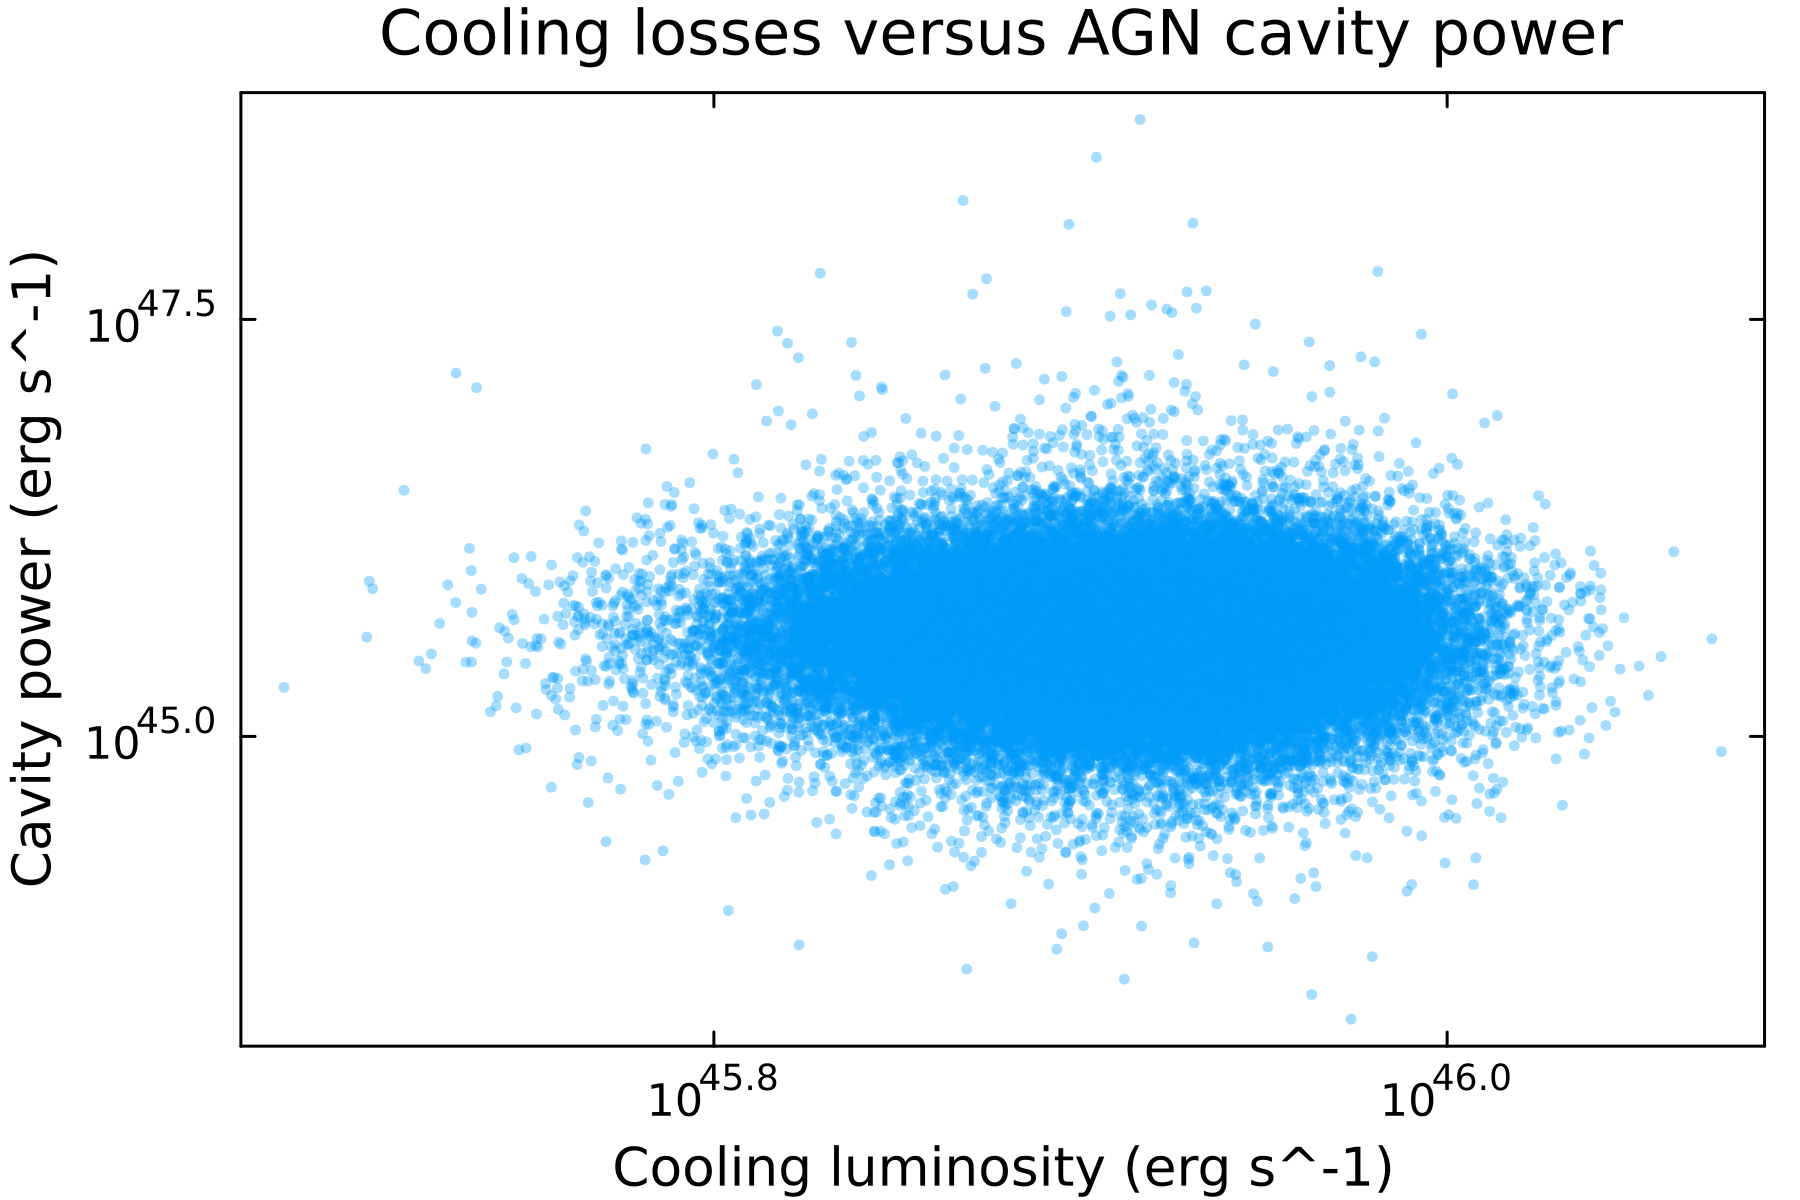
\includegraphics[width=\columnwidth]{../figures/cooling_vs_feedback.pdf}
\caption{Cooling luminosity versus cavity power for individual Monte Carlo
  samples (log-log scale). The correlation structure arises from shared parameter
  dependencies.}
\label{fig:scatter}
\end{figure}

\begin{figure*}[htbp]
\centering
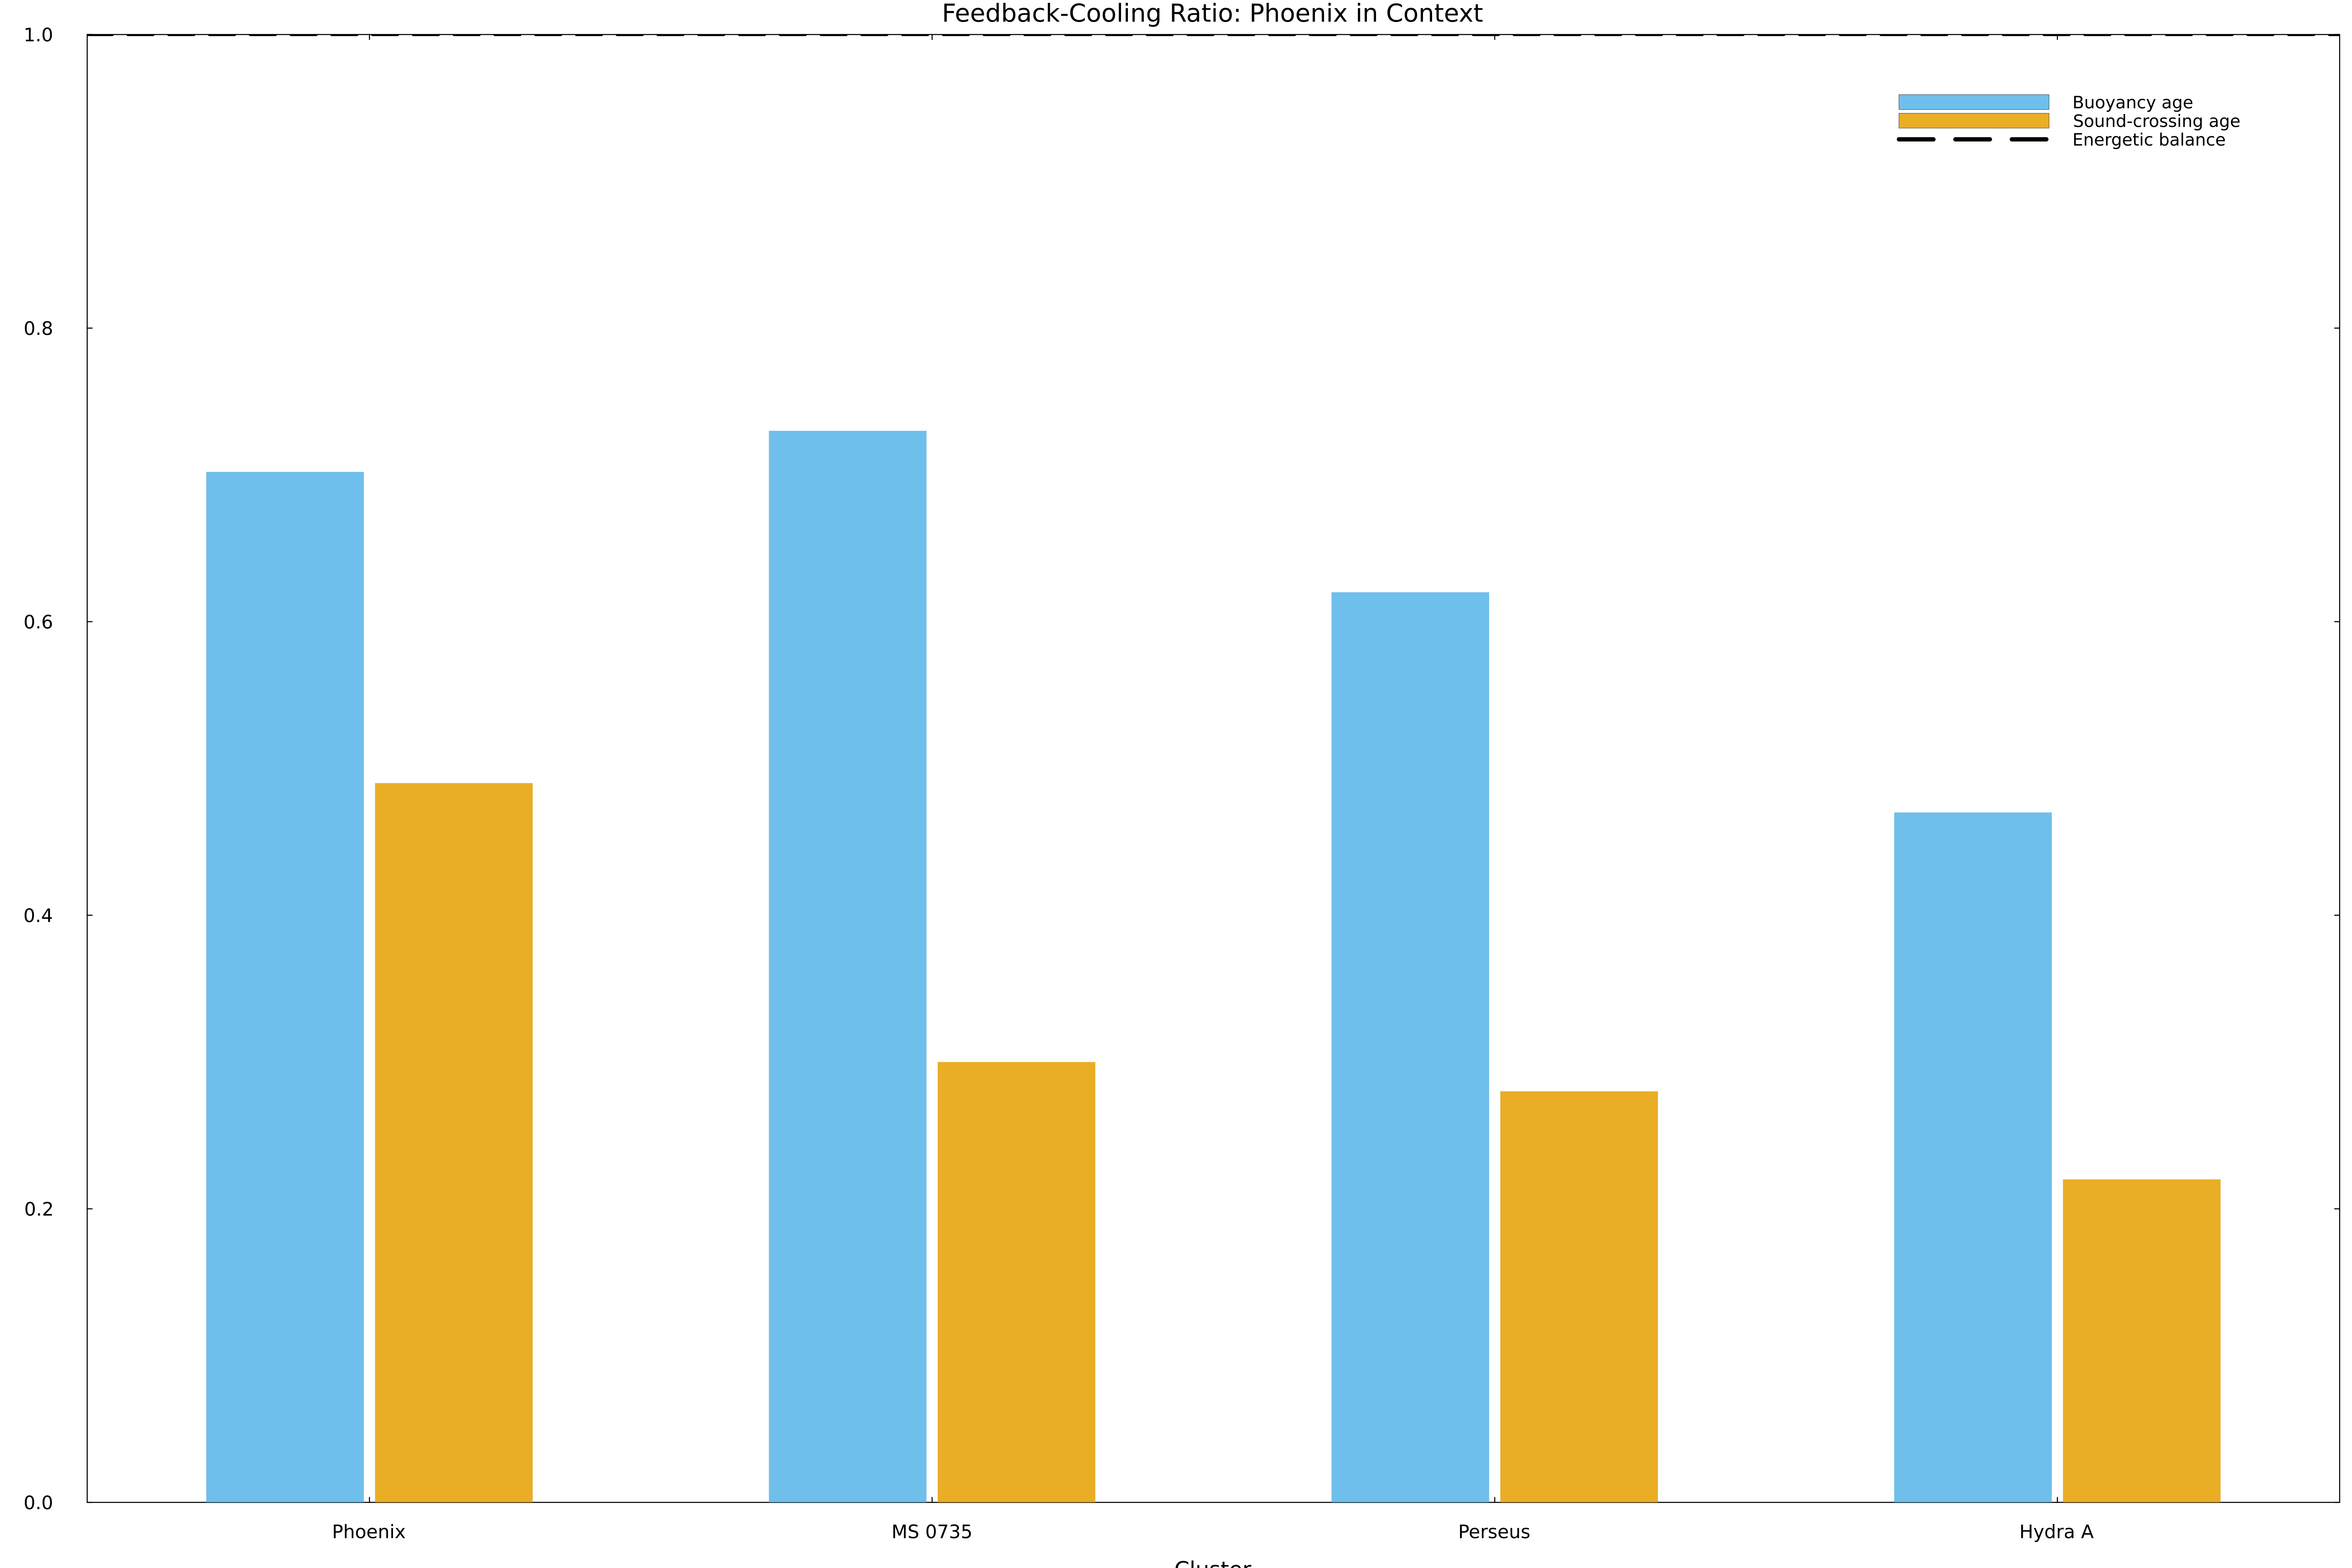
\includegraphics[width=\textwidth]{../figures/cluster_comparison.pdf}
\caption{Feedback-cooling ratio comparison across four well-studied cool-core
  clusters (Phoenix, MS~0735, Perseus, Hydra~A) for buoyancy-age and
  sound-crossing-age estimates. The dashed line marks energetic balance.
  Phoenix's ratio is comparable to MS~0735 under buoyancy-age assumptions but
  its extreme absolute cooling rate makes the residual cooling far more
  significant.}
\label{fig:clustercomp}
\end{figure*}

\begin{figure*}[htbp]
\centering
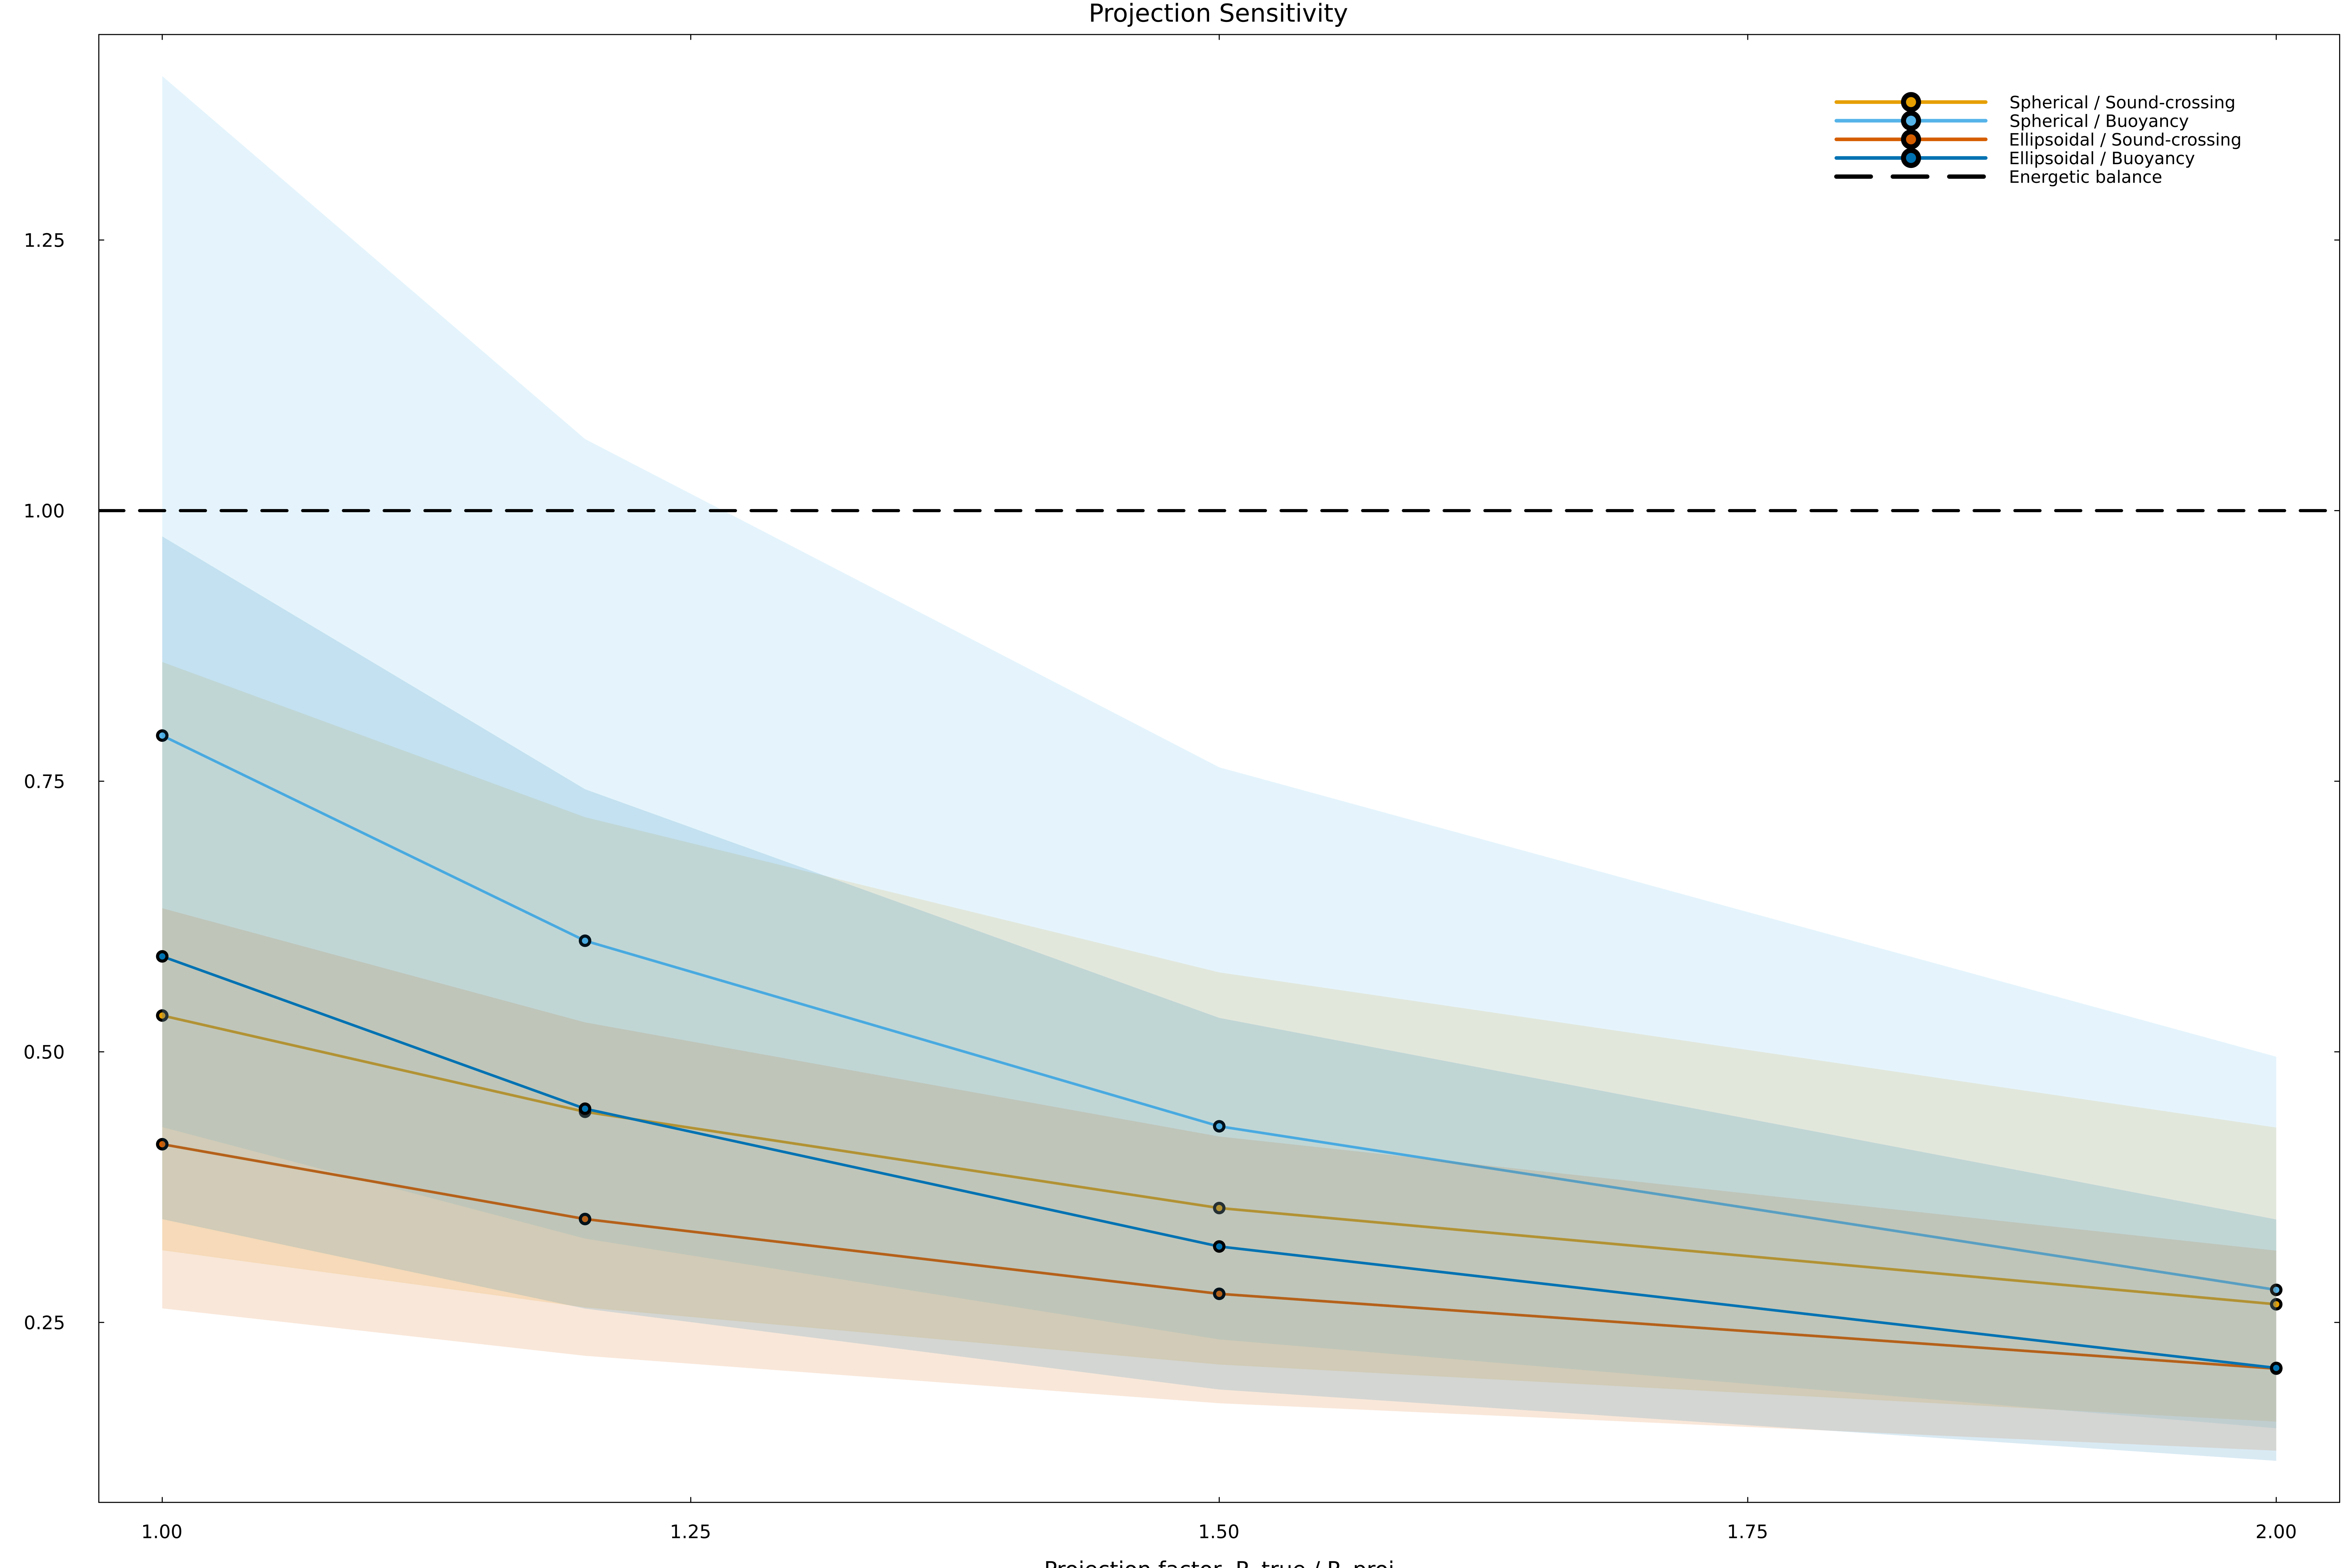
\includegraphics[width=\textwidth]{../figures/projection_sensitivity.pdf}
\caption{Projection sensitivity of the feedback ratio. The observed cavity
  distance $R$ is a projected quantity; the true three-dimensional distance may
  be larger by a factor $f$. Curves show the median and 16th--84th percentile
  range for each model as $f$ varies from 1.0 (no correction) to 2.0.
  Higher projection factors increase the dynamical ages and therefore decrease
  the inferred cavity power and feedback ratio.}
\label{fig:proj}
\end{figure*}

% =============================================================================
% -- Input parameters table ---------------------------------------------------

\begin{deluxetable*}{lllll}
\tablecaption{Input assumption parameters\label{tab:inputs}}
\tablehead{
\colhead{Parameter} & \colhead{Value} & \colhead{Uncertainty} &
\colhead{Aperture} & \colhead{Source}
}
\startdata
$\Lcool$ ($\erg\;\s^{-1}$) & $8.2 \times 10^{45}$ & $\pm 10\%$ &
  $r < 100\;\kpc$, 0.7--7.0~keV & \citet{McDonald2012, McDonald2019} \\
$kT$ ($\keV$) & 5.9 & $\pm 12\%$ & 10--30~kpc & \citet{McDonald2019} \\
$n_e$ ($\cm^{-3}$) & 0.12 & $\pm 15\%$ & $r < 10\;\kpc$ & \citet{McDonald2019} \\
$\pcav$ ($\erg\;\cm^{-3}$) & $1.5 \times 10^{-9}$ & $\pm 25\%$ &
  cavity location & \citet{McDonald2015} \\
$\rcav$ ($\kpc$) & 12 & $\pm 20\%$ & projected & \citet{McDonald2015} \\
$a$ ($\kpc$) & 14 & $\pm 20\%$ & major axis & \citet{Hlavacek-Larrondo2015} \\
$b$ ($\kpc$) & 9 & $\pm 25\%$ & minor axis & \citet{Hlavacek-Larrondo2015} \\
$R$ ($\kpc$) & 25 & $\pm 20\%$ & projected distance & \citet{McDonald2015} \\
\enddata
\tablecomments{Full citation audit with exact table/figure references in
  \codeloc{paper/tables/literature\_values.md}.}
\end{deluxetable*}

% =============================================================================
% -- ApJ-required metadata ----------------------------------------------------

\section*{Acknowledgments}

We thank Michael McDonald, Brian McNamara, Julie Hlavacek-Larrondo, and their
collaborators for making the \textit{Chandra}, ALMA, and \textit{XMM-Newton}
data for the Phoenix Cluster publicly available, and for the detailed cavity
measurements and thermodynamic profiles that form the foundation of this
analysis. This research has made use of data obtained from the Chandra Data
Archive. This research received no external funding. The author acknowledges the
use of advanced AI models in the development of this analysis framework.

\section*{Data Availability}

The Julia pipeline, Monte Carlo simulation code, and all input data used in this
analysis are publicly available at
\url{https://github.com/phanendra09/phoenix-cluster-feedback}. The
\textit{Chandra} X-ray data used to derive the input parameters are available
from the Chandra Data Archive (\url{https://cda.harvard.edu/chaser/}). No
proprietary data are used in this analysis. All results, including the full Monte
Carlo samples, are included in the repository.

\facility{Chandra (ACIS), ALMA}

\software{Julia 1.12.6 (\url{https://julialang.org}), CSV.jl, DataFrames.jl,
  JSON.jl, Plots.jl, LaTeXStrings.jl, ProgressMeter.jl, Random.jl, SHA.jl,
  Statistics.jl, Test.jl. Full version-pinned dependencies are recorded in
  \texttt{Manifest.toml} in the repository.}

\section*{Reproducibility}

All results in this paper were generated with a single command:
\begin{verbatim}
julia --project=. scripts/run_pipeline.jl --full --seed 42
\end{verbatim}
This runs $50{,}000$ Monte Carlo samples (seed 42), all six age/geometry model
combinations, the sensitivity grid, and produces all figures and summary tables.
Pipeline metadata (including input file SHA-256 hash, git commit, Julia version,
timestamps, and the full command line) is recorded in
\texttt{results/run\_metadata.json}. Dependency versions are pinned in
\texttt{Manifest.toml}.

% =============================================================================
\bibliography{references}
\bibliographystyle{aasjournal}

\end{document}
